\documentclass[12pt]{report}

% margins
\usepackage[top=1.0in, bottom=1.0in, left=1.5in, right=1.0in]{geometry}
%\usepackage[top=1.0in, bottom=1.2in, left=1.7in, right=1.0in]{geometry}

% langue
\usepackage[T1]{fontenc}
\usepackage[utf8]{inputenc}
\usepackage[french]{babel}

% double spacing
\usepackage{setspace}
\onehalfspacing

% graphics and subfigures
\usepackage{graphicx}
\usepackage[captionskip=8pt, nearskip=10pt]{subfig}
\usepackage{float}
\usepackage{lscape}
\usepackage{placeins}

% couleur officielle Université Paris-Saclay (prune, Pantone 229C)
\usepackage{xcolor}
\definecolor{saclayprune}{HTML}{63003C}

% en-têtes / pieds de page
\usepackage{fancyhdr}

% mise en forme des titres de chapitre/section
\usepackage{titlesec}

% citations
\usepackage{cite}

% abbreviations
\usepackage{nomencl}
\makenomenclature

% math
\usepackage{amsmath}
\usepackage{amssymb}

% algorithms
\usepackage{algorithm}
\usepackage{algorithmic}

%definitions
\newtheorem {myDef} {Définition}
\newtheorem{myEx}{Exemple}
\newcommand{\tabincell}[2]{\begin{tabular}{@{}#1@{}}#2\end{tabular}}

% capitalize names of sections
\def\contentsname{TABLE DES MATIÈRES}
\def\listtablename{LISTE DES TABLEAUX}
\def\listfigurename{LISTE DES FIGURES}
\def\transparencystatementname{DÉCLARATION DE TRANSPARENCE}
\def\bibname{RÉFÉRENCES}
\addto\captionsfrench{%
  \renewcommand{\tablename}{Tableau}%
  \renewcommand{\figurename}{Figure}%
}

% numérotation des chapitres en chiffres romains (Partie I, II, III...)
\renewcommand{\thechapter}{\Roman{chapter}}

% élargit la boîte réservée au numéro dans la table des matières :
% "III" et "VI" sont plus larges que le 1.5em par défaut de report.cls,
% ce qui les faisait toucher le titre du chapitre sans espace
\makeatletter
\renewcommand*\l@chapter[2]{%
  \ifnum \c@tocdepth >\m@ne
    \addpenalty{-\@highpenalty}%
    \vskip 1.0em \@plus\p@
    \setlength\@tempdima{2.6em}%
    \begingroup
      \parindent \z@ \rightskip \@pnumwidth
      \parfillskip -\@pnumwidth
      \leavevmode \bfseries
      \advance\leftskip\@tempdima
      \hskip -\leftskip
      #1\nobreak\hfil \nobreak\hb@xt@\@pnumwidth{\hss #2}\par
      \penalty\@highpenalty
    \endgroup
  \fi}
\makeatother

% titres de chapitre et de section dans la couleur officielle
\titleformat{\chapter}[display]
  {\normalfont\bfseries}
  {\Large\color{saclayprune}\chaptertitlename\ \thechapter}
  {14pt}
  {\huge\color{saclayprune}}
  [\vspace{2pt}{\color{saclayprune}\titlerule[1pt]}]
\titlespacing*{\chapter}{0pt}{10pt}{28pt}
\titleformat{\section}
  {\normalfont\Large\bfseries\color{saclayprune}}
  {\thesection}{0.8em}{}
\titleformat{\subsection}
  {\normalfont\large\bfseries\color{saclayprune}}
  {\thesubsection}{0.8em}{}

% en-tête : chapitre courant · pied de page : numéro
\pagestyle{fancy}
\fancyhf{}
\renewcommand{\headrulewidth}{0.4pt}
\renewcommand{\footrulewidth}{0pt}
\fancyhead[L]{\small\textit{\nouppercase{\leftmark}}}
\fancyhead[R]{\small\thepage}
\fancypagestyle{plain}{%
  \fancyhf{}
  \fancyfoot[C]{\small\thepage}
  \renewcommand{\headrulewidth}{0pt}
}

% chemin des figures : décommentez/adaptez selon l'organisation de votre
% projet Overleaf (les 4 images .png doivent être uploadées dans le projet)
\graphicspath{{./}{../}}

\title{Agrégation des Préférences Utilisateur sous Contraintes d'Équité, de Diversité et d'Inclusion par Résumé de Graphe}
\author{Adji Marieme Sita Cissé}
\date{2026}

\begin{document}

\pagenumbering{roman}

\begin{titlepage}
\centering
\vspace*{0.5cm}
\includegraphics[width=0.5\textwidth]{logo-paris-saclay}\\[1.1cm]

{\large Master 2 DataScale\\}
{\large Université Paris-Saclay (UVSQ)\\[0.3cm]}
{\small en séjour de recherche au\\
Department of Computer Science, University of Regina\par}

\vfill

{\color{saclayprune}\rule{\linewidth}{1.2pt}}\\[0.7cm]
{\Large\bfseries Agrégation des Préférences Utilisateur\\[0.25cm]
sous Contraintes d'Équité, de Diversité et d'Inclusion\\[0.25cm]
par Résumé de Graphe\\[0.6cm]}
{\color{saclayprune}\rule{\linewidth}{1.2pt}}

\vfill

{\large\bfseries Mémoire de stage}

\vfill

\begin{minipage}{0.33\textwidth}
\centering
{\large\textbf{Auteure}}\\[2pt]
\normalsize Adji Marieme Sita Cissé
\end{minipage}%
\begin{minipage}{0.33\textwidth}
\centering
{\large\textbf{Encadrant}}\\[2pt]
\normalsize Prof. Malek Mouhoub
\end{minipage}%
\begin{minipage}{0.33\textwidth}
\centering
{\large\textbf{Tutrice pédagogique}}\\[2pt]
\normalsize Zoubida Kedad
\end{minipage}

\vspace{1.5cm}
{\large 2026}
\vspace*{0.5cm}
\end{titlepage}

\tableofcontents
\listoffigures
\listoftables
\clearpage
\pagenumbering{arabic}

\chapter*{Préface}
\addcontentsline{toc}{chapter}{Préface}
\markboth{Préface}{Préface}
\label{chap:preface}

\section*{Résumé}
\addcontentsline{toc}{section}{Résumé}

L'agrégation des préférences de groupes d'utilisateurs divers en un résultat
collectif soulève des défis fondamentaux d'équité, de diversité et
d'inclusion (EDI) : les règles d'agrégation classiques telles que Borda et
Condorcet ne disposent d'aucun mécanisme empêchant les résultats de
favoriser systématiquement les groupes majoritaires, de converger vers des
items homogènes, ou de sous-représenter les minorités. Ces tensions se
manifestent concrètement dans la recommandation collective, où
l'optimisation de la seule utilité renforce le biais majoritaire et les
bulles de filtres. Nous abordons ce problème par le résumé de graphe sous
contraintes EDI. Les préférences des utilisateurs sont modélisées comme un
graphe biparti attribué et pondéré, et un algorithme de \emph{coarsening}
glouton fusionne itérativement des nœuds utilisateurs tout en imposant
trois critères structurels d'EDI : une contrainte d'écart d'équité
($\Delta E$), une contrainte de diversité intra-liste (ILD), et une
contrainte d'inclusion de groupe. Plutôt que de corriger l'équité après
l'agrégation, notre méthode intègre la préservation de l'EDI directement
dans la structure du graphe.

Nous évaluons notre approche sur cinq jeux de données couvrant quatre
domaines --- recommandation de films (MovieLens 100k et 1M), rencontres
sociales (libimseti.cz), évaluation pédagogique (Rate My Professors), et
paternité académique en IA/ML/informatique (OpenAlex, 2018--2023). Aucune
méthode de référence ne satisfait simultanément les trois critères EDI à
travers tous les domaines. Notre méthode, AURORA, obtient les gains de
diversité les plus importants et les plus constants par rapport aux règles
de vote classiques (Borda, Borda pondéré, Condorcet), et sur MovieLens
100k à $k=20$, elle améliore simultanément les trois critères EDI par
rapport à Borda et à Condorcet. Dans les configurations d'équité côté
item, elle combine de façon unique une forte diversité (ILD$=0{,}808$)
avec la meilleure représentation féminine des items
($\mathrm{frac}_F=60\,\%$) sur Rate My Professors --- au prix toutefois
d'un coût d'équité modéré par rapport à Borda sur ce jeu de données --- et
atteint l'écart d'équité le plus faible ($\Delta E=0{,}051$) sur OpenAlex,
où les méthodes fondées sur Borda ne recommandent aucune autrice. Sur
libimseti.cz, seul jeu de données où l'attribut sensible est présent des
deux côtés du graphe biparti, aucune méthode ne réduit l'écart d'équité
--- une limite que nous analysons et relions à des travaux antérieurs
montrant que la parité démographique n'est pas toujours une cible
d'équité appropriée lorsque les préférences diffèrent réellement entre
les groupes. Ces résultats démontrent que l'intégration de contraintes
EDI dans la structure d'agrégation produit des compromis
équité--diversité plus robustes que les approches a posteriori, tout en
révélant qu'aucun budget de compression ni mécanisme structurel unique ne
résout la tension équité--diversité de manière uniforme à travers les
domaines.

\bigskip
\noindent\textbf{Mots-clés :} coarsening de graphe, systèmes de
recommandation, équité algorithmique, métriques EDI, agrégation de
préférences, graphe biparti, choix social.

\section*{Remerciements}
\addcontentsline{toc}{section}{Remerciements}

Je remercie le Prof. Malek Mouhoub pour son encadrement tout au long de
ce stage, ainsi que Zoubida Kedad pour son suivi pédagogique. Je
souhaite également remercier ma famille pour son soutien constant : mes
parents, mes tantes et tous mes oncles, tout particulièrement Mayata
Ndiaye Mbaye. Merci aussi à Abdoulaye Dahirou Dia, ainsi qu'à Serigne
Amouyakar Fall, pour son soutien moral et sa présence. J'ai une pensée
particulière pour mon défunt oncle et ami Alioune Ndoye, qui n'a cessé
de prier pour moi.

\chapter{Contexte du Stage}
\label{chap:contexte}

\section{Établissement d'accueil}

Ce stage de recherche s'est déroulé au sein du \textbf{Department of
Computer Science} de l'\textbf{University of Regina} (Saskatchewan,
Canada), dans le cadre d'un séjour de recherche à l'international
s'inscrivant dans le Master 2 DataScale de l'Université Paris-Saclay
(UVSQ), financé par la \textbf{bourse de mobilité Data IA}. Le stage a
été encadré par le \textbf{Prof. Malek Mouhoub}, enseignant-chercheur
au sein de ce département et responsable du \textbf{Constraint
Processing Lab}, le laboratoire de recherche d'accueil.

\section{Missions du Département}

Le Department of Computer Science de l'University of Regina mène des
activités de recherche et d'enseignement en informatique. Le
\emph{Constraint Processing Lab}, dirigé par le Prof. Malek Mouhoub,
couvre notamment l'optimisation multi-objectif, l'aide à la décision
multicritère, l'apprentissage automatique, la planification des
horaires de personnel (infirmiers et autres effectifs), la
planification de mouvement et de trajectoire pour robots, les tournées
de véhicules et le transport, l'aménagement urbain, la sécurité de
l'Internet des objets (IoT), et l'élaboration d'emplois du temps
(\emph{timetabling}). C'est dans ce contexte, à l'intersection de
l'optimisation multi-objectif et de l'aide à la décision, que
s'inscrit la problématique de l'équité algorithmique traitée durant ce
stage.

\section{Origine du Sujet de Recherche}

Le sujet de recherche, portant sur l'équité, la diversité et
l'inclusion (EDI) dans les systèmes de recommandation, a été proposé
par le Prof. Malek Mouhoub et développé de façon autonome durant le
stage. Il a donné lieu à la rédaction d'un article scientifique soumis
à une conférence internationale (format Springer LNCS), dont ce
mémoire reprend et détaille le contenu en français. Le suivi
pédagogique côté Université Paris-Saclay a été assuré par Zoubida
Kedad.

\chapter{Objectif du Stage}
\label{chap:objectif}

\section{Ma Mission dans le Projet}

L'idée de départ de ce projet vient du Prof. Malek Mouhoub : explorer le
résumé de graphe (\emph{graph summarization}) comme moyen de traiter les
enjeux d'équité, de diversité et d'inclusion (EDI) dans l'agrégation de
préférences utilisateur. Au-delà de cette idée initiale, l'intégralité de
la conception, du développement et de l'évaluation a été réalisée de
façon autonome durant ce stage : la formalisation du problème et des
métriques EDI, la conception de l'algorithme de \emph{coarsening} sous
contraintes, son implémentation, la mise en place du protocole
expérimental sur cinq jeux de données, l'analyse des résultats, ainsi que
le nom donné à la méthode, \textbf{AURORA}\footnote{\emph{Attributed
Unified gRaph cOarsening for equitable RecommendAtion.} Le choix de ce
nom fait aussi écho aux aurores boréales observées pendant le séjour de
recherche à Regina, en Saskatchewan.}, ont été menés seule.

\section{Le Problème Traité}

À mesure que les systèmes algorithmiques médiatisent de plus en plus
l'accès à l'information, aux opportunités et aux ressources, garantir que
leurs résultats ne désavantagent pas systématiquement certains groupes
est devenu une préoccupation centrale dans de nombreux domaines, du
recrutement au crédit en passant par la curation de
contenu~\cite{mehrabi2021survey}. Les
systèmes de recommandation illustrent concrètement cette tension : leur
objectif traditionnel, maximiser l'utilité prédite pour chaque
utilisateur, tend à renforcer les items déjà populaires (effet Matthieu)
et à enfermer les utilisateurs dans des bulles de filtres homogènes. Ces
effets soulèvent des préoccupations d'équité, de diversité et d'inclusion
(EDI) : les recommandations collectives peuvent favoriser
systématiquement les goûts des groupes majoritaires, offrir peu de
variété, et sous-représenter les minorités.

Traiter l'EDI en recommandation nécessite d'agréger les préférences de
nombreux utilisateurs en un résultat collectif tout en traitant les
groupes équitablement. Les approches existantes assurent généralement
l'équité en modifiant les préférences en entrée~\cite{kamiran2012data},
en modifiant le
classement en sortie par re-classement~\cite{singh2018fairness}, ou en
régularisant l'algorithme
d'apprentissage~\cite{zhao_fairness_2024}. Le résumé de graphe, de son côté, offre un moyen
puissant de réduire de grands graphes de préférences en représentations
compactes, mais il a traditionnellement été guidé par la fidélité
structurelle ou l'efficacité, jamais par la préservation de l'équité.

\section{Objectif}

L'objectif de ce stage était de combler cette lacune : représenter les
préférences utilisateur comme un graphe biparti attribué et pondéré, et
concevoir une méthode de résumé de graphe --- AURORA --- qui réduit la
taille de ce graphe tout en préservant explicitement trois propriétés :
l'équité, la diversité, et l'inclusion. L'approche devait ensuite être
comparée à cinq règles d'agrégation classiques (Average Score, Borda,
Borda pondéré, Condorcet, Fair Re-rank) et évaluée sur plusieurs jeux de
données couvrant des domaines et des configurations de biais différents,
afin de vérifier si la méthode généralise au-delà d'un unique cas
favorable. Le détail de cette démarche est présenté aux
chapitres~\ref{chap:etat-art} à~\ref{chap:validation}.

\chapter{État de l'Art}
\label{chap:etat-art}

\section{Notions Préliminaires}
\label{sec:background}

Cette section introduit les concepts et notations utilisés tout au long de
ce mémoire : le graphe de préférences, l'agrégation de préférences, le
résumé de graphe, et les notions d'équité, de diversité et d'inclusion.

\subsection{Graphe de préférences}

Nous représentons les données de préférences comme un graphe biparti
attribué et pondéré
\[
  G = (U \cup I,\; E,\; w,\; s),
\]
où $U = \{u_1, \ldots, u_m\}$ est l'ensemble des nœuds utilisateurs, $I =
\{i_1, \ldots, i_n\}$ est l'ensemble des nœuds items (par exemple des
films, des professeurs, ou des chercheurs), et $E \subseteq U \times I$
est l'ensemble des arêtes. Une arête $(u, i) \in E$ existe si et seulement
si l'utilisateur $u$ a noté l'item $i$. La fonction de poids $w : E
\rightarrow [1, 5]$ donne la note attribuée par $u$ à $i$. L'attribut
sensible $s$ est défini sur les nœuds utilisateurs dans les configurations
d'\emph{équité côté utilisateur} ($s : U \rightarrow \{F, M\}$, par
exemple MovieLens, libimseti) ou sur les nœuds items dans les
configurations d'\emph{équité côté item} ($s : I \rightarrow \{F, M\}$,
par exemple Rate My Professors, OpenAlex), où $\{F, M\}$ désigne les deux
groupes de genre. Le graphe est biparti : les arêtes relient uniquement
des utilisateurs à des items, jamais deux utilisateurs ou deux items entre
eux.

\subsection{Agrégation de préférences}

L'agrégation de préférences est la tâche consistant à combiner les
préférences individuelles de nombreux utilisateurs en un résultat
collectif unique, typiquement un classement ou un ensemble top-$k$
d'items~\cite{ricci2011recommender}. Les règles d'agrégation classiques
constituent nos méthodes de référence. Le \emph{score moyen} classe les
items selon leur note moyenne ; le \emph{compte de Borda} convertit les
notes de chaque utilisateur en rangs et les additionne ; le \emph{Borda
pondéré} normalise les scores de Borda par la taille des groupes pour
compenser les déséquilibres démographiques ; et la méthode de
\emph{Condorcet} compare les items par paires, un item l'emportant si une
majorité d'utilisateurs le préfère. Aucune de ces règles ne contrôle
explicitement l'EDI pendant l'agrégation, ce qui motive l'approche
proposée dans ce mémoire.

\subsection{Résumé de graphe}

Le résumé de graphe réduit un grand graphe à une représentation plus
petite qui préserve certaines propriétés sélectionnées de l'original. Nous
nous concentrons sur la famille du regroupement (ou agrégation), dans
laquelle les nœuds sont fusionnés en \emph{super-nœuds} selon leur
similarité, et les arêtes entre groupes sont agrégées en
\emph{super-arêtes}~\cite{liu_graph_2018}. Le processus de fusion de
nœuds pour obtenir un graphe plus petit est appelé \emph{coarsening}. Le
résumé obtenu est plus petit et plus rapide à traiter, mais la fusion
élimine nécessairement de l'information ; la question centrale est donc de
savoir quelles propriétés le résumé doit préserver.

\subsection{Équité, diversité et inclusion}

Nous considérons trois notions distinctes, désignées conjointement par
EDI. L'\emph{équité} désigne le traitement juste des groupes définis par
l'attribut sensible, de sorte qu'aucun groupe ne soit systématiquement
favorisé ou désavantagé par le résultat collectif --- que le groupe soit
défini sur les utilisateurs (équité côté utilisateur) ou sur les items
recommandés (équité côté item). La \emph{diversité} désigne la variété des
items recommandés, en évitant les listes dominées par un seul type ou par
les items les plus populaires. L'\emph{inclusion} désigne le fait de
garantir que les groupes minoritaires soient représentés dans le résultat
au moins en proportion de leur taille. Ces trois notions sont distinctes
et peuvent être en tension : améliorer l'une peut dégrader une autre.
Notre travail les traite comme des propriétés à préserver lors du résumé
du graphe de préférences, et les métriques précises utilisées pour les
quantifier sont définies au chapitre~\ref{chap:approche}.

\section{Revue de la Littérature}
\label{sec:litreview}

Notre travail se situe à l'intersection de quatre domaines de recherche :
l'agrégation de préférences et le choix social, le résumé de graphe,
l'équité algorithmique (équité, diversité et inclusion), et les systèmes
de recommandation sensibles à l'équité. Nous passons chacun en revue,
puis identifions la lacune que notre contribution comble.

\subsection{Agrégation de Préférences et Choix Social}

L'agrégation de préférences --- combiner les préférences de nombreux
utilisateurs en un résultat collectif --- est étudiée en théorie du choix
social computationnel. Roy et al.~\cite{roy_fairness_2024} structurent le
problème selon trois dimensions (format d'entrée, format de sortie,
règle d'agrégation) et rappellent le théorème d'impossibilité d'Arrow :
aucune règle ne peut satisfaire simultanément un ensemble raisonnable de
critères d'équité, ce qui motive de raisonner en \emph{propriétés
préservées} plutôt qu'en règle optimale unique. Ils distinguent
notamment rendre un résultat équitable en modifiant les préférences en
entrée, de le rendre équitable en modifiant le classement en sortie ---
une opposition à laquelle nous revenons pour positionner notre approche.
Kellerhals et Peters~\cite{kellerhals_proportional_2024} relient le
clustering proportionnel au vote multi-gagnants et montrent que
plusieurs notions d'équité peuvent être satisfaites simultanément ; leur
analyse opère sur une métrique de graphe, regroupant les nœuds en
clusters équitables --- conceptuellement proche du résumé d'un graphe de
préférences sous garanties d'équité.

\subsection{Résumé de Graphe (État de l'Art)}

Liu et al.~\cite{liu_graph_2018} fournissent la revue de référence du
domaine et organisent les méthodes en quatre familles : regroupement
(fusion de nœuds en super-nœuds), compression de bits,
simplification/parcimonisation, et approches fondées sur l'influence.
Leur constat central : il n'existe pas de définition unique d'un
\emph{bon} résumé, sa qualité dépendant de l'objectif visé --- une
observation directement pertinente ici, puisque notre graphe porte un
attribut sensible et est donc un graphe étiqueté. Shabani et
al.~\cite{shabani_comprehensive_2024}, plus récents, appliquent les
réseaux de neurones sur graphes au résumé et identifient le résumé
\emph{orienté tâche} (adapté à un besoin aval précis, plutôt que
générique) comme direction de recherche ouverte. Notre travail
s'inscrit dans la famille regroupement/agrégation et répond directement
à cette direction : notre critère de qualité du résumé est la
préservation de l'équité, de la diversité et de l'inclusion.

\subsection{EDI dans les Systèmes de Recommandation et l'Équité Algorithmique}

Yao et Huang~\cite{yao_new_2017} montrent que la parité démographique est
souvent inappropriée en filtrage collaboratif, les préférences dépendant
réellement d'attributs sensibles comme le genre ; nous reprenons leur
métrique de \emph{value unfairness} pour notre écart d'équité $\Delta E$.
Leonhardt et al.~\cite{leonhardt_user_2018} apportent une preuve
empirique d'un compromis direct entre diversité et équité utilisateur :
augmenter la diversité accroît sensiblement la disparité entre
utilisateurs. Zhao et al.~\cite{zhao_fairness_2024} passent en revue
équité et diversité conjointement, classant les techniques en pré-, in-
et post-traitement, et formulent le problème comme une optimisation
multi-objectif sur un front de Pareto. Dong et
al.~\cite{dong_fairness_2023}, le domaine le plus proche d'AURORA,
montrent que les graphes posent des défis d'équité absents des données
i.i.d. (biais structurel par homophilie) ; parmi leurs techniques de
mitigation, l'\emph{edge rewiring} est la seule à agir sur la structure
du graphe comme AURORA --- mais en ajoutant/retirant des arêtes, alors que
nous réduisons le graphe par fusion de nœuds.

\subsection{Choix Social pour la Recommandation Sensible à l'Équité}

Aird et al.~\cite{aird_exploring_2023} introduisent SCRUF-D : chaque
préoccupation d'équité y est modélisée comme un agent qui vote (Borda,
Copeland, Ranked Pairs) aux côtés du système de recommandation de base pour produire
le classement final. Une extension~\cite{aird_social_2024} généralise ce
cadre à l'équité hétérogène. C'est le travail conceptuellement le plus
proche d'AURORA, et pourtant fondamentalement différent : SCRUF-D agit au
moment de produire le classement final --- un post-traitement --- alors
qu'AURORA agit en amont, sur la structure du graphe résumé, avant même que
le classement ne soit calculé. Leur exploration approfondie de la voie
post-hoc laisse la voie structurelle ouverte.

\subsection{Lacune de Recherche}

À travers ces quatre domaines, un constat cohérent se dégage. L'équité en
recommandation a surtout été traitée par modification des entrées ou des
sorties, par pré-, intra-, ou post-traitement, ou par \emph{edge
rewiring} sur la structure du graphe ; le résumé de graphe, de son côté,
a traditionnellement optimisé la fidélité structurelle, le stockage, la
vitesse de requête, ou le débruitage. À notre connaissance, aucun travail
existant ne fait de la préservation de l'équité, de la diversité et de
l'inclusion un critère de qualité explicite d'un résumé de graphe. C'est
précisément la lacune que notre travail comble. Nous étudions donc la
question de recherche suivante : étant donné un graphe biparti pondéré de
préférences, comment construire un résumé, par détection de communautés
et \emph{coarsening}, qui réduit sa taille tout en bornant la dégradation
de l'équité, de la diversité et de l'inclusion, par rapport aux règles
d'agrégation classiques ?

\chapter{Approche Suivie et Solution Proposée}
\label{chap:approche}
\label{sec:methodology}

En nous appuyant sur le modèle de graphe et le contexte introduits au
chapitre~\ref{chap:etat-art}, ce chapitre définit précisément les trois
métriques EDI, formule l'objectif de résumé sous contraintes, et décrit
comment nous dérivons un classement collectif à partir du graphe résumé.

\section{Métriques EDI}

Soit $R = (r_1, \ldots, r_k)$ un classement collectif top-$k$ produit à
partir du graphe de préférences, et soient $\mathcal{G}_F, \mathcal{G}_M
\subset U$ les deux groupes d'utilisateurs induits par l'attribut sensible
$s$.

\smallskip\noindent\textbf{Équité.}
Nous mesurons l'équité par la métrique de \emph{value unfairness} de Yao
et Huang~\cite{yao_new_2017}. Pour chaque groupe $g \in \{F, M\}$,
l'utilité de groupe sur la liste top-$k$ est
\begin{equation}
  \mathrm{utility}_g(R)
    = \frac{1}{|\mathcal{G}_g|}
      \sum_{u \in \mathcal{G}_g}
      \frac{1}{k} \sum_{i \in R} w(u, i),
\end{equation}
où $w(u,i)=0$ lorsque $(u,i)\notin E$. L'écart d'équité est alors
\begin{equation}
  \Delta E(R) = \bigl|\mathrm{utility}_F(R) - \mathrm{utility}_M(R)\bigr|.
\end{equation}
Une valeur de $\Delta E$ proche de zéro indique que les deux groupes
retirent une satisfaction moyenne similaire du résultat collectif.

\smallskip\noindent\textbf{Diversité.}
Nous mesurons la diversité par la métrique de diversité intra-liste
(ILD) :
\begin{equation}
  \mathrm{ILD}(R) = \frac{2}{k(k-1)}
    \sum_{\substack{i,j \in R \\ i \neq j}} \mathrm{dist}(i,j),
\end{equation}
où $\mathrm{dist}(i,j) = 1 - \mathrm{cosine}(\mathbf{v}_i, \mathbf{v}_j)$
et $\mathbf{v}_i \in \mathbb{R}^m$ est le vecteur de notes de l'item $i$
sur l'ensemble des utilisateurs, avec $\mathbf{v}_i[u] = w(u,i)$ si
$(u,i)\in E$ et $0$ sinon. Une ILD plus élevée indique une liste de
recommandation plus variée.

\smallskip\noindent\textbf{Inclusion.}
Nous mesurons l'inclusion par un critère d'équité proportionnelle fondé
sur le concept central de Kellerhals et
Peters~\cite{kellerhals_proportional_2024} et opérationnalisé comme la
métrique d'équité proportionnelle de groupe d'Aird et
al.~\cite{aird_social_2024}. Soit $\theta$ un seuil de pertinence et
$\alpha_g = |\mathcal{G}_g|/|U|$ la part de population du groupe $g$. Le
score d'inclusion du groupe $g$ est
\begin{equation}
  \mathrm{inclusion}_g(R)
    = \frac{1}{|\mathcal{G}_g|}
      \sum_{u \in \mathcal{G}_g}
      \frac{|\{i \in R : w(u,i) \geq \theta\}|}{k}.
\end{equation}
L'inclusion est satisfaite pour le groupe $g$ lorsque
$\mathrm{inclusion}_g(R) \geq \alpha_g$ : un groupe représentant
$\alpha_g$ de la population d'utilisateurs devrait trouver au moins la
même proportion d'items top-$k$ pertinents. Nous fixons $\theta = 4{,}0$
par défaut et comparons avec $\theta = 3{,}5$ expérimentalement.

\paragraph{Équité côté item.}
Dans les configurations d'équité côté item (Rate My Professors,
OpenAlex), l'attribut sensible est défini sur les items plutôt que sur
les utilisateurs. La métrique d'inclusion principale est alors la
fraction d'items féminins dans la liste top-$k$ :
\[
  \mathrm{frac}_F(R) = \frac{|\{i \in R : s(i) = F\}|}{k}.
\]
L'écart d'équité $\Delta E$ est adapté en conséquence, comparant
l'utilité moyenne reçue par les items féminins et masculins sur
l'ensemble des utilisateurs du graphe.

\section{Résumé de Graphe sous Contraintes EDI}

Plutôt que d'imposer l'EDI comme une correction a posteriori sur un
classement déjà calculé, notre approche intègre la préservation de l'EDI
directement dans le processus de \emph{coarsening}. Chaque fusion
candidate de nœuds utilisateurs n'est acceptée que si le graphe résumé
résultant maintient l'écart d'équité, la diversité intra-liste, et
l'inclusion de groupe du graphe original dans des tolérances prescrites.
Cette intégration structurelle garantit que l'équité n'est pas sacrifiée
à la compression après coup, mais préservée à mesure que le graphe est
progressivement réduit.

\smallskip\noindent\textbf{Coarsening.}
En partant de $G = (U \cup I, E, w, s)$, nous fusionnons itérativement des
paires de nœuds utilisateurs en super-nœuds selon la similarité de leurs
profils de notation. Le résultat est un graphe résumé $G' = (U' \cup I,
E', w', s')$ avec $|U'| < |U|$, où chaque super-nœud $S \subseteq U$
représente un groupe d'utilisateurs originaux. Le poids agrégé du
super-nœud $S$ vers l'item $i$ est
\begin{equation}
  w'(S, i) =
    \frac{\displaystyle\sum_{u \in S:\,(u,i)\in E} w(u,i)}
         {|\{u \in S : (u,i) \in E\}|},
\end{equation}
lorsqu'au moins un membre de $S$ a noté $i$. Le classement collectif
top-$k$ est ensuite dérivé de $G'$ à l'aide des règles d'agrégation
décrites en section~\ref{sec:background}. Le nombre de fusions acceptées
est borné par un budget de fusion exprimé comme une fraction de $|U|$
plutôt qu'un compte absolu, de sorte que la même cible de compression
relative s'applique quelle que soit la taille du jeu de données ; le
chapitre~\ref{chap:validation} rapporte un balayage de robustesse
sur ce budget.

\smallskip\noindent\textbf{Contraintes de préservation EDI.}
Une fusion produisant le résumé candidat $G'$ est acceptée si et
seulement si
\begin{align}
  \Delta E(G') &\leq \Delta E(G) + \varepsilon_E, \\
  \mathrm{ILD}(G') &\geq \mathrm{ILD}(G) - \varepsilon_D, \\
  \mathrm{inclusion}_g(G') &\geq \mathrm{inclusion}_g(G) - \varepsilon_I
  \quad \forall\, g,
\end{align}
où $\varepsilon_E, \varepsilon_D, \varepsilon_I \geq 0$ sont des
tolérances de dégradation contrôlant le compromis entre compression et
préservation de l'EDI.

\smallskip\noindent\textbf{Objectif formel.}
Le problème global s'écrit
\begin{equation}
\begin{aligned}
  \min_{G'} \quad & \mathcal{L}(G, G') \\
  \text{s.c.} \quad
    & \Delta E(G') \leq \Delta E(G) + \varepsilon_E, \\
    & \mathrm{ILD}(G') \geq \mathrm{ILD}(G) - \varepsilon_D, \\
    & \mathrm{inclusion}_g(G') \geq \mathrm{inclusion}_g(G) - \varepsilon_I
      \quad \forall\, g,
\end{aligned}
\end{equation}
où $\mathcal{L}(G, G')$ est la perte structurelle mesurée comme l'erreur
quadratique moyenne entre les poids d'arêtes originaux et reconstruits.
Les tolérances sont calibrées empiriquement à partir de mesures de
référence sur le graphe complet, comme décrit au
chapitre~\ref{chap:validation}.

\section{Exemple Illustratif}

Pour illustrer concrètement comment une agrégation non contrainte peut
nuire à l'EDI, considérons quatre utilisateurs --- $u_1 \in \mathcal{G}_F$
et $u_2, u_3, u_4 \in \mathcal{G}_M$ --- et trois items, avec des notes
présentées au tableau~\ref{tab:toy}. Ce ratio 1F:3M reflète le
déséquilibre de genre du jeu de données MovieLens 100k (29\,\% de femmes,
71\,\% d'hommes), notre principal benchmark d'évaluation.

Classer les items par score moyen donne $i_2 \succ i_3 \succ i_1$, car
$i_1$ est noté 5 par $u_1$ mais seulement 1 et 2 par deux utilisateurs
masculins, ce qui abaisse sa moyenne à 2,67. La recommandation top-2 $R =
\{i_2, i_3\}$ expose un problème d'équité sévère. En calculant les
métriques EDI sur $R$ (avec $\theta = 4$) :
\begin{align*}
  \mathrm{utility}_F(R) &= \tfrac{1}{2}(w(u_1,i_2)+w(u_1,i_3))
                         = \tfrac{1}{2}(2+0) = 1{,}0, \\
  \mathrm{utility}_M(R) &= \tfrac{1}{6}\sum_{j=2}^{4}(w(u_j,i_2)+w(u_j,i_3))
                         = \tfrac{26}{6} = 4{,}33, \\
  \Delta E(R) &= |1{,}0 - 4{,}33| = 3{,}33.
\end{align*}
De plus, $u_1$ ne trouve aucun item dans $R$ avec $w(u_1,i) \geq 4$, donc
$\mathrm{inclusion}_F(R) = 0 < \alpha_F = 0{,}25$, tandis que
$\mathrm{inclusion}_M(R) = 0{,}83 > \alpha_M = 0{,}75$ : l'utilisatrice
est entièrement exclue des items pertinents de la liste top-2.

Si $i_1$ avait été inclus à la place --- $R' = \{i_1, i_2\}$ --- nous
obtiendrions $\Delta E(R') = 0{,}67$ et $\mathrm{inclusion}_F(R') = 0{,}5
\geq \alpha_F$ : un résultat nettement plus équitable. Notre
\emph{coarsening} sous contraintes EDI détecte de telles distorsions au
niveau structurel : toute fusion de nœuds utilisateurs qui conduirait à
recommander $R$ plutôt que $R'$ est rejetée, car elle augmente $\Delta E$
au-delà de la tolérance $\varepsilon_E$.

\begin{table}[H]
\centering
\caption{Exemple jouet : notes (-- désigne une entrée non observée).}
\label{tab:toy}
\begin{tabular}{lcccc}
\hline
Utilisateur & Groupe & $i_1$ & $i_2$ & $i_3$ \\
\hline
$u_1$ & F & 5  & 2  & --  \\
$u_2$ & M & 1  & 5  & 3   \\
$u_3$ & M & -- & 4  & 5   \\
$u_4$ & M & 2  & 5  & 4   \\
\hline
\end{tabular}
\end{table}

\chapter{Validation}
\label{chap:validation}
\label{sec:experimentation}

\section{Jeux de Données}

Nous évaluons notre approche sur cinq jeux de données couvrant quatre
domaines, recouvrant à la fois des configurations d'équité côté
utilisateur et côté item.

\paragraph{MovieLens 100k et 1M~\cite{harper2015movielens}.}
MovieLens 100k contient 100~000 notes de 943 utilisateurs sur 1~682
films (échelle 1--5). Le genre est l'attribut sensible sur les
utilisateurs : $\mathcal{G}_F$ (273 femmes, 29\,\%) et $\mathcal{G}_M$
(670 hommes, 71\,\%). MovieLens 1M étend ce jeu de données à 6~040
utilisateurs, 3~706 films, et 1~000~209 notes, utilisé pour valider le
passage à l'échelle. Nous fixons $k \in \{5, 10, 20\}$.

\paragraph{libimseti.cz.}
Un réseau social de rencontres tchèque où les utilisateurs notent
d'autres utilisateurs sur leur attractivité. L'attribut sensible est le
genre de l'utilisateur qui note (équité côté utilisateur). Nous utilisons
$k = 10$.

\paragraph{Rate My Professors.}
Une plateforme d'évaluation pédagogique où les étudiants notent des
professeurs. L'attribut sensible est le genre du professeur (équité côté
item). Nous utilisons $k = 10$.

\paragraph{OpenAlex (IA/ML/informatique, 2018--2023).}
Un graphe de paternité académique construit à partir de l'API OpenAlex,
comprenant 99 venues, 904 auteurs (171 F / 733 M, $\alpha_F \approx
19\,\%$), et 2~124 notes (comptes de co-paternité). Le genre est déduit
du prénom de l'auteur. L'attribut sensible est sur les items (équité côté
item). Nous utilisons $k = 10$.

\begin{figure}[H]
\centering
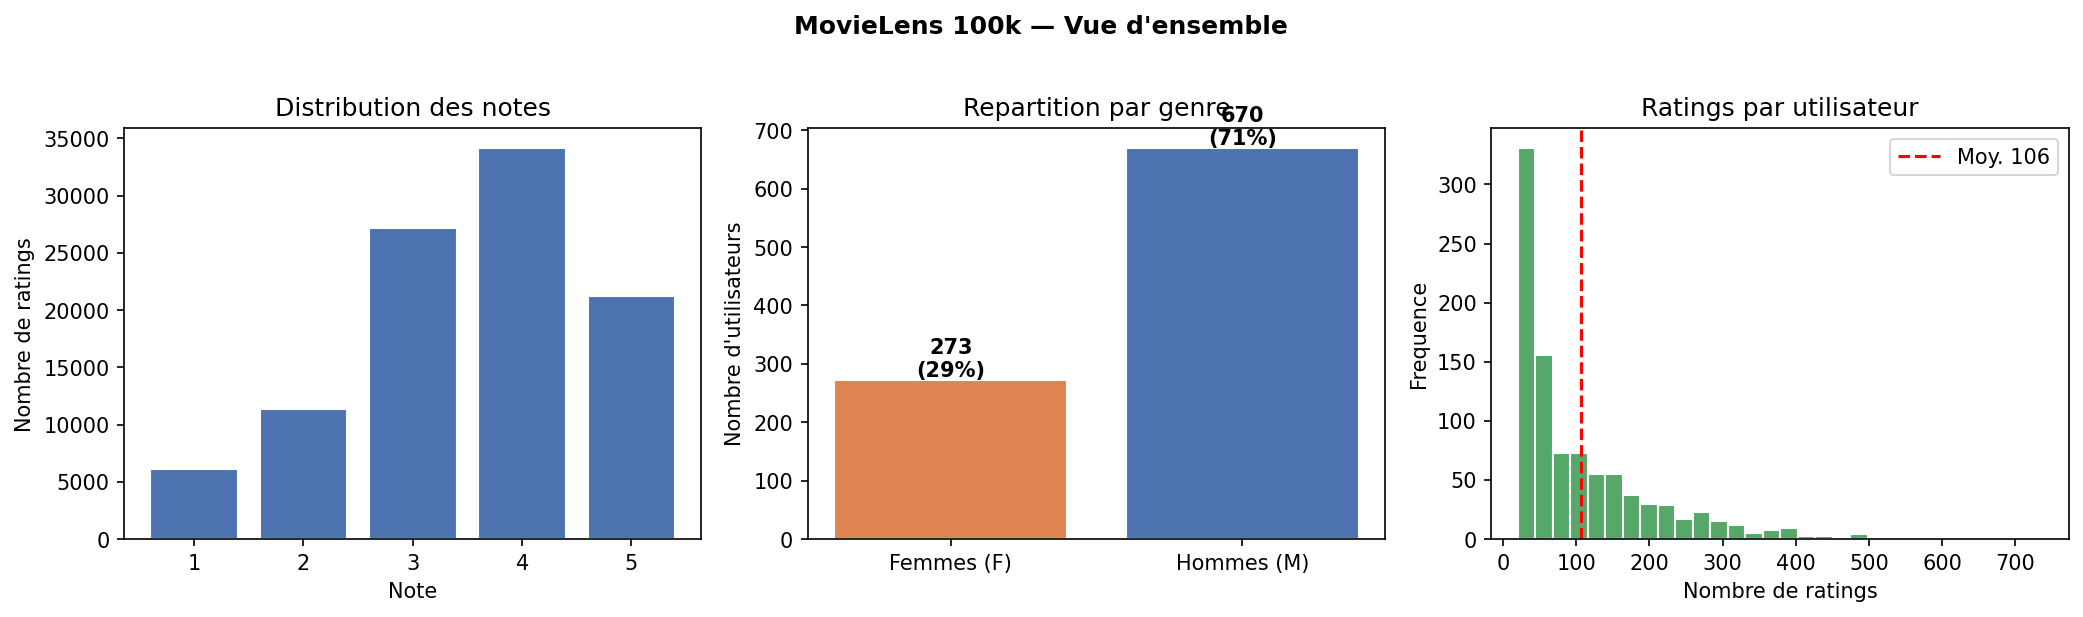
\includegraphics[width=\textwidth]{fig_data_overview_fr}
\caption{Vue d'ensemble de MovieLens 100k : distribution des notes,
répartition par genre (273 F / 670 M), et nombre de notes par
utilisateur.}
\label{fig:data}
\end{figure}

\section{Méthodes de Référence}

Nous comparons notre résumé sous contraintes EDI à cinq méthodes de
référence : (1)~\textbf{Average Score}, qui classe les items par leur
note moyenne ; (2)~\textbf{Borda Count}, qui convertit les notes de
chaque utilisateur en rangs et les additionne ; (3)~\textbf{Weighted
Borda}, qui normalise les scores de Borda par la taille des groupes pour
compenser les déséquilibres démographiques ; (4)~\textbf{Condorcet}, qui
classe les items par préférence majoritaire par paires ; et
(5)~\textbf{Fair Re-rank}, une méthode de post-traitement qui re-classe
de façon gloutonne les 40 meilleurs candidats de Borda pour maximiser la
somme des scores d'inclusion de groupe tout en minimisant l'écart
d'équité. Aucune des quatre premières règles ne contrôle explicitement
l'EDI pendant l'agrégation ; Fair Re-rank traite l'EDI comme une
correction a posteriori.

\section{Protocole d'Évaluation}

Nous évaluons toutes les méthodes sur les métriques EDI définies en
section~\ref{sec:methodology}. Pour les jeux de données à équité côté
utilisateur (MovieLens, libimseti), nous rapportons $\Delta E$, l'ILD, et
les scores d'inclusion de groupe ($\mathrm{inc}_F$, $\mathrm{inc}_M$),
avec un seuil de pertinence $\theta \in \{3{,}5, 4{,}0\}$ pour MovieLens.
Pour les jeux de données à équité côté item (Rate My Professors,
OpenAlex), nous rapportons $\Delta E$, l'ILD, et $\mathrm{frac}_F$ --- la
fraction d'items féminins dans la liste top-$k$. Les tolérances de
dégradation sont fixées à $\varepsilon_E = 0{,}1$, $\varepsilon_D =
0{,}05$, et $\varepsilon_I = 0{,}05$, calibrées à partir de mesures de
référence sur le graphe complet. Nous fixons $k \in \{5, 10, 20\}$ pour
MovieLens et $k = 10$ pour tous les autres jeux de données, et rapportons
le taux de compression $|U'|/|U|$ aux côtés de toutes les métriques EDI.

\section{Résultats}

Le tableau~\ref{tab:k10} rapporte les métriques EDI et le taux de
compression pour toutes les méthodes à $k=10$, $\theta=4{,}0$ ; les
mêmes tendances s'observent à $k=5$ et $k=20$ (détails ci-dessous).

\begin{table}[h!]
\centering
\caption{Métriques EDI à $k=10$, $\theta=4{,}0$. \textbf{Gras} : meilleure
valeur par colonne. $\alpha_F=0{,}29$, $\alpha_M=0{,}71$.}
\label{tab:k10}
\begin{tabular}{lccccc}
\hline
Méthode & $\Delta E\downarrow$ & ILD$\uparrow$ & $\mathrm{inc}_F\uparrow$
       & $\mathrm{inc}_M\uparrow$ & Ratio$\downarrow$ \\
\hline
Average Score & \textbf{0,007} & \textbf{1,000} & 0,001 & 0,002 & -- \\
Borda         & 0,425 & 0,354 & 0,293 & 0,392 & -- \\
Weighted Borda & 0,425 & 0,354 & 0,293 & 0,392 & -- \\
Condorcet     & 0,446 & 0,356 & 0,292 & 0,394 & -- \\
Fair Re-rank  & 0,162 & 0,429 & 0,271 & 0,313 & -- \\
AURORA          & 0,423 & 0,391 & \textbf{0,307} & \textbf{0,405} & \textbf{0,499} \\
\hline
Cible $\alpha_g$ & -- & -- & 0,29 & 0,71 & -- \\
\hline
\end{tabular}
\end{table}

Trois constats principaux se dégagent. \textbf{Average Score} obtient le
plus faible $\Delta E$ et la plus haute ILD, mais c'est un résultat
\emph{dégénéré} : la méthode recommande les mêmes items à tout le monde,
indépendamment du groupe, donc son inclusion est quasi nulle --- elle ne
distingue simplement jamais les utilisateurs. \textbf{Fair Re-rank}
obtient systématiquement le meilleur $\Delta E$ parmi les méthodes qui
distinguent réellement les groupes, confirmant qu'un post-traitement
ciblé réduit efficacement l'écart d'équité. \textbf{AURORA} bat les trois
règles de vote classiques (Borda, Weighted Borda, Condorcet) sur
$\Delta E$ à chaque $k \in \{5,10,20\}$, tout en obtenant le meilleur
score d'inclusion pour au moins un groupe à chaque $k$ ; c'est la seule
méthode à améliorer les quatre métriques par rapport à Borda
simultanément à $k=10$. Sur l'ILD, elle dépasse Borda
et Condorcet à presque tous les $k$ (seule exception : $k=5$, où
Condorcet est légèrement au-dessus), et rattrape Fair Re-rank à $k=20$
(0,462 contre 0,427) sans y parvenir à $k=5$ et $k=10$. Enfin, le taux de
compression d'AURORA reste stable autour de 50\,\% quel que soit $k$,
car le budget de fusion est exprimé en fraction de $|U|$ plutôt qu'en
valeur absolue --- un choix validé par un balayage de robustesse en
section~\ref{sec:robustness}.

\begin{figure}[h!]
\centering
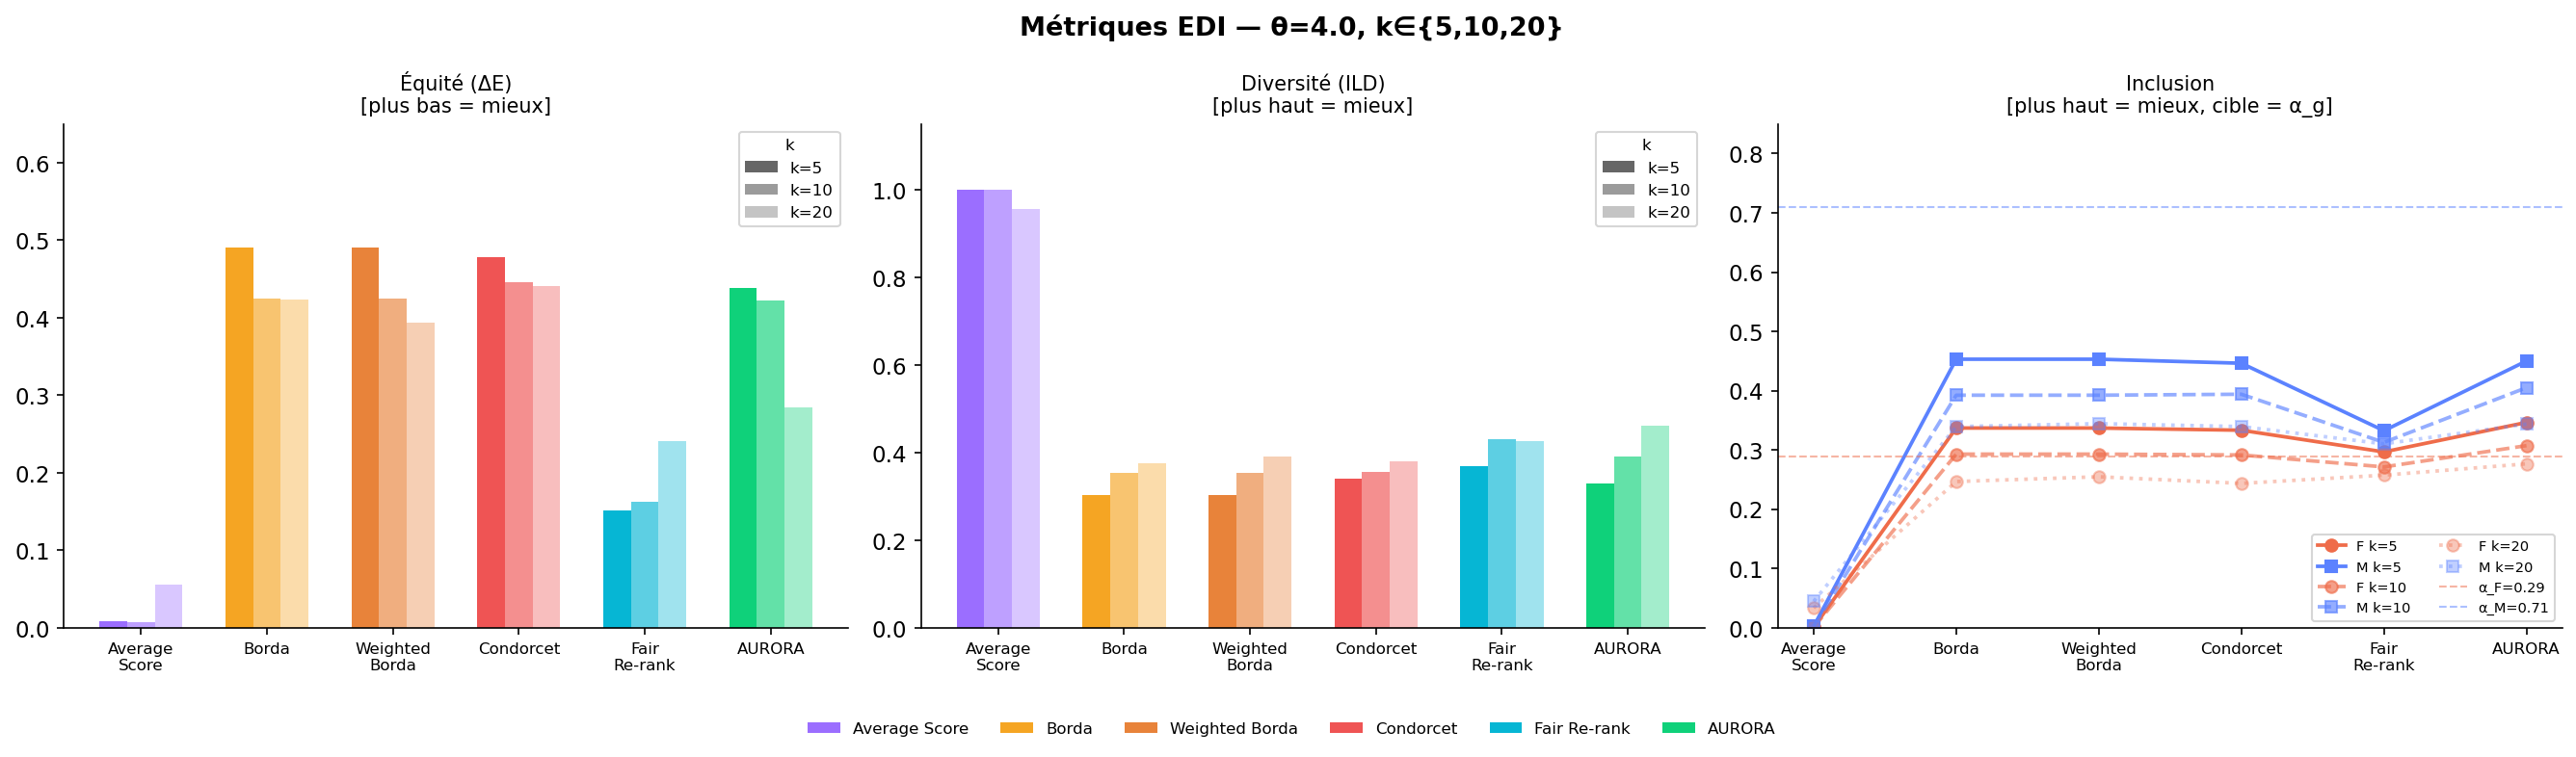
\includegraphics[width=\textwidth]{fig_edi_baselines}
\caption{Métriques EDI pour toutes les méthodes de référence à $k \in
\{5, 10, 20\}$, $\theta = 4{,}0$. Un $\Delta E$ plus bas est meilleur
(équité) ; une ILD plus haute est meilleure (diversité) ; une inclusion
plus haute est meilleure, les lignes pointillées marquant les cibles
proportionnelles $\alpha_F=0{,}29$ et $\alpha_M=0{,}71$.}
\label{fig:baselines}
\end{figure}

\begin{table}[h!]
\caption{Temps d'exécution moyen (secondes) par méthode et taille de
         liste $k$, mesuré sur MovieLens 100k ($\theta = 4{,}0$, moyenné
         sur 3 exécutions).}
\label{tab:runtime}
\centering
\begin{tabular}{lrrr}
\hline
\textbf{Méthode} & \textbf{k = 5} & \textbf{k = 10} & \textbf{k = 20} \\
\hline
Average Score  &   0,005\,s &   0,004\,s &   0,004\,s \\
Borda          &   0,720\,s &   0,677\,s &   0,666\,s \\
Weighted Borda & ${\sim}0{,}72$ s & ${\sim}0{,}68$ s & ${\sim}0{,}67$ s \\
Condorcet      &   0,149\,s &   0,129\,s &   0,126\,s \\
Fair Re-rank   &   0,938\,s &   0,928\,s &   0,926\,s \\
\textbf{AURORA}  & \textbf{3,793\,s} & 3,761\,s &   4,042\,s \\
\hline
\end{tabular}
\end{table}

\paragraph{Efficacité computationnelle.}
Le tableau~\ref{tab:runtime} rapporte les temps d'exécution par méthode.
Toutes les méthodes de référence s'exécutent en moins d'une seconde,
tandis qu'AURORA prend 3,8 à 4,0\,s sur MovieLens 100k --- environ 4 à 6
fois plus lent que Fair Re-rank et 5 à 6 fois plus lent que Borda.
Ce temps reste stable quel que soit $k$ (le budget de fusion, exprimé en
fraction de $|U|$, ne dépend pas de $k$), et demeure de l'ordre de
quelques secondes même sur un jeu de données plus grand
(section~\ref{sec:scalability}) --- acceptable puisque le
\emph{coarsening} est typiquement effectué hors ligne, avant toute
recommandation en temps réel.

\section{Évaluation Multi-Domaines}

Les tableaux~\ref{tab:libimseti}--\ref{tab:oalex} étendent l'évaluation
aux trois jeux de données supplémentaires.

Sur \textbf{libimseti} (tableau~\ref{tab:libimseti}, $\theta=7{,}0$ sur
l'échelle 1--10 de la plateforme), Average Score reste dégénéré (même
mécanisme que ci-dessus) et Fair Re-rank est le seul à obtenir un
$\Delta E$ bas (0,144) parmi les méthodes non dégénérées ; AURORA obtient
la meilleure ILD (0,761) mais, comme les méthodes de vote, ne réduit pas
$\Delta E$ (au-delà de 1,2). Cette limite --- propre à ce seul jeu de
données --- est analysée en détail en
section~\ref{sec:libimseti-limitation} : elle reflète une réelle
différence de comportement de notation entre groupes plutôt qu'une
lacune algorithmique, et persiste même en faisant varier le budget de
fusion de 30\,\% à 60\,\% de $|U|$.

Sur \textbf{Rate My Professors} (tableau~\ref{tab:rmp}), AURORA obtient
la deuxième meilleure diversité (ILD$=0{,}808$) et la meilleure
représentation de professeures ($\mathrm{frac}_F=0{,}60$), au prix d'un
$\Delta E$ (0,112) plus élevé que Borda (0,008) : sur ce corpus, la
méthode échange une part d'équité contre un net gain de diversité et de
représentation. Fair Re-rank monte $\mathrm{frac}_F$ à 0,50 mais avec une
diversité bien plus faible (ILD$=0{,}196$), montrant que le re-classement
a posteriori ne peut pas optimiser diversité et représentation aussi
bien que le \emph{coarsening} structurel.

Sur \textbf{OpenAlex} (tableau~\ref{tab:oalex}), le déséquilibre est
extrême : Borda, Weighted Borda et Condorcet recommandent \emph{zéro}
autrice, bien que les femmes représentent 19\,\% des auteurs. AURORA
obtient ici le meilleur des deux mondes : le plus faible $\Delta E$
(0,051, 28\,\% de mieux qu'Average Score) tout en maintenant une
représentation féminine comparable ($\mathrm{frac}_F=0{,}197$) ---
contrairement à RMP, elle améliore équité \emph{et} diversité
simultanément, confirmant que la méthode généralise à d'autres
configurations d'équité côté item, avec des bénéfices qui restent
toutefois dépendants du domaine.

\begin{table}[h!]
\caption{Métriques EDI sur libimseti.cz ($k=10$, équité côté utilisateur,
$\theta=7{,}0$ sur l'échelle 1--10 de la plateforme). Gras : meilleur par
colonne.}
\label{tab:libimseti}
\centering
\begin{tabular}{lcccc}
\hline
Méthode & $\Delta E \downarrow$ & ILD $\uparrow$ &
$\mathrm{inc}_F \uparrow$ & $\mathrm{inc}_M \uparrow$ \\
\hline
Average Score  & \textbf{0,016} & \textbf{0,867} & 0,002 & 0,000 \\
Borda          & 1,218 & 0,744 & 0,147 & \textbf{0,024} \\
Weighted Borda & 1,218 & 0,744 & 0,147 & \textbf{0,024} \\
Condorcet      & 1,296 & 0,746 & \textbf{0,157} & \textbf{0,024} \\
Fair Re-rank   & 0,144 & 0,719 & 0,039 & \textbf{0,024} \\
AURORA           & 1,232 & 0,761 & 0,148 & \textbf{0,024} \\
\hline
\end{tabular}
\end{table}

\section{Pourquoi $\Delta E$ Reste Élevé sur libimseti}
\label{sec:libimseti-limitation}

Sur les trois autres jeux de données, l'attribut sensible ne réside que
d'un seul côté du graphe biparti : le genre est une propriété des
utilisateurs sur MovieLens, et une propriété des items sur Rate My
Professors et OpenAlex. libimseti est différent : les évaluateurs et les
profils évalués portent tous deux une étiquette de genre, car les items
recommandés sont eux-mêmes des personnes. Pour comprendre pourquoi aucune
méthode --- y compris AURORA --- ne réduit $\Delta E$ ici, nous avons
croisé la note moyenne par paire de genre (évaluateur, profil évalué) sur
l'ensemble du graphe (12~258~052 notes avec genre connu des deux côtés) :
les femmes notent les hommes 6,92/10 en moyenne, les hommes notent les
femmes 5,48/10, et les notes entre personnes du même genre sont plus
basses encore (5,14 pour F$\to$F, 4,46 pour M$\to$M). Cet écart est
constant sur plus de 12 millions de notes : c'est une propriété
structurelle des données, pas du bruit statistique.

Un classement collectif unique, partagé par tous indépendamment du
groupe, ne peut pas satisfaire des évaluateurs dont les distributions de
notes diffèrent autant. Cela explique pourquoi $\Delta E$ reste élevé
pour les méthodes de vote et pour AURORA (Average Score et Fair Re-rank
n'y échappent que parce qu'elles ne différencient jamais les groupes) :
la contrainte de préservation EDI du \emph{coarsening} n'a ici
essentiellement aucun effet, car fusionner des utilisateurs du même
genre ne peut pas transférer d'information sur les préférences d'un
groupe pour des profils qu'il note structurellement plus bas.

Ce résultat illustre empiriquement un argument de Yao et
Huang~\cite{yao_new_2017} : la parité démographique n'est pas toujours
une cible d'équité appropriée lorsque les préférences de groupes
différents divergent réellement. Sur MovieLens ou Rate My Professors,
rien ne suggère que le genre devrait influencer l'appréciation d'un film
ou la note d'un professeur, donc un $\Delta E$ persistant y est
vraisemblablement dû à la règle d'agrégation. Sur libimseti, en
revanche, l'attribut sensible entre dans la préférence elle-même via la
structure de l'attraction romantique, donc un $\Delta E$ élevé peut
refléter une différence réelle plutôt qu'un résultat à corriger. Ce
constat tient quel que soit le budget de fusion testé
(section~\ref{sec:robustness}) : nous le considérons comme une limite
réelle de tout cadre à classement unique sur ce type de domaine, plutôt
qu'un défaut spécifique à notre méthode.

\begin{table}[h!]
\caption{Métriques EDI sur Rate My Professors ($k=10$, équité côté item).
$\mathrm{frac}_F$ = fraction de professeures dans le top-$k$.
Gras : meilleur par colonne.}
\label{tab:rmp}
\centering
\begin{tabular}{lccc}
\hline
Méthode & $\Delta E \downarrow$ & ILD $\uparrow$ &
$\mathrm{frac}_F \uparrow$ \\
\hline
Average Score  & \textbf{0,000} & \textbf{0,982} & 0,40 \\
Borda          & 0,008 & 0,145 & 0,40 \\
Weighted Borda & 0,008 & 0,145 & 0,40 \\
Condorcet      & 0,076 & 0,253 & 0,30 \\
Fair Re-rank   & \textbf{0,000} & 0,196 & 0,50 \\
AURORA           & 0,112 & 0,808 & \textbf{0,60} \\
\hline
\end{tabular}
\end{table}
\FloatBarrier
\begin{table}[h!]
\caption{Métriques EDI sur OpenAlex IA/ML/informatique 2018--2023
($k=10$, équité côté item ; $\alpha_F \approx 19\,\%$). Gras : meilleur
par colonne.}
\label{tab:oalex}
\centering
\begin{tabular}{lccc}
\hline
Méthode & $\Delta E \downarrow$ & ILD $\uparrow$ &
$\mathrm{frac}_F \uparrow$ \\
\hline
Average Score  & 0,071 & \textbf{0,356} & \textbf{0,200} \\
Borda          & 1,233 & 0,000 & 0,000 \\
Weighted Borda & 1,233 & 0,000 & 0,000 \\
Condorcet      & 1,233 & 0,000 & 0,000 \\
Fair Re-rank   & 0,071 & \textbf{0,356} & \textbf{0,200} \\
AURORA           & \textbf{0,051} & 0,351 & 0,197 \\
\hline
\end{tabular}
\end{table}
\FloatBarrier

\section{Robustesse au Budget de Fusion}
\label{sec:robustness}

Le budget de fusion (section~\ref{sec:methodology}) est fixé à 50\,\% de
$|U|$ tout au long des expériences principales. Pour vérifier que ce
choix n'est pas un réglage étroit et sélectionné après coup, nous
ré-exécutons AURORA à quatre budgets (30\,\%, 42,4\,\%, 50\,\%, 60\,\% de
$|U|$) sur MovieLens 1M et Rate My Professors, les deux jeux de données
où l'effet de la compression est le plus visible.

Sur MovieLens~1M, AURORA bat les trois règles de vote à la fois sur
$\Delta E$ et sur l'ILD sur toute cette plage, et les deux métriques
s'améliorent légèrement quand le budget augmente ($\Delta E$ : 0,332 à
30\,\% $\to$ 0,185 à 60\,\% ; ILD : 0,456 $\to$ 0,470) --- la méthode est
robuste au choix exact du budget. Sur Rate My Professors, l'ILD reste
stable et élevée (0,75--0,81) sur toute la plage, confirmant que le gain
de diversité n'est pas un artefact du réglage à 50\,\% ; $\Delta E$, en
revanche, ne s'améliore pas de façon monotone avec la compression (ce
que nous attribuons à la granularité grossière d'un classement à
$k=10$), et reste dans tous les cas supérieur à celui de Borda
($\approx 0{,}008$) : le compromis équité/diversité décrit en
section~\ref{sec:libimseti-limitation} tient quel que soit le budget
choisi entre 30 et 60\,\%.

\subsection*{Synthèse Inter-Domaines}

Le tableau~\ref{tab:synthesis} résume la méthode la plus performante par
métrique et par jeu de données. AURORA est en tête sur la diversité
(MovieLens 100k) et sur la diversité \emph{et} la représentation côté
item (RMP, OpenAlex), et bat chaque règle de vote classique sur
$\Delta E$ partout. Elle n'est cependant pas la meilleure méthode
partout : Fair Re-rank la surpasse sur les deux axes sur MovieLens 1M.
Aucune méthode ne l'emporte sur toutes les métriques et tous les
domaines, confirmant que les objectifs EDI sont en tension et qu'aucun
mécanisme --- structurel ou a posteriori --- ne domine uniformément.

\begin{table}[h!]
\caption{Synthèse inter-domaines : meilleure méthode par métrique à
$k=10$ (ou le $k$ unique rapporté pour libimseti, RMP, OpenAlex).}
\label{tab:synthesis}
\centering
\footnotesize
\resizebox{\textwidth}{!}{%
\begin{tabular}{@{}lllll@{}}
\hline
Jeu de données & Meilleur $\Delta E$ & Meilleure ILD & Meilleure
inc/frac$_F$ & Globale \\
\hline
ML 100k  & Fair Re-rank & Fair Re-rank & \textbf{AURORA} & \textbf{AURORA} ($k{=}20$) \\
ML 1M    & Fair Re-rank & Fair Re-rank & Fair Re-rank & Fair Re-rank \\
libimseti & Fair Re-rank & \textbf{AURORA} & Condorcet & Aucune (écart persistant) \\
RMP      & Avg Score / F.R. & Avg Score & \textbf{AURORA} & Compromis : AURORA (div.) / F.R. (éq.) \\
OpenAlex & \textbf{AURORA} & Avg Score / F.R. & Avg Score / F.R. & \textbf{AURORA} \\
\hline
\end{tabular}%
}
\par\smallskip
\footnotesize $^*$Average Score est exclue quand elle est dégénérée sur
l'inclusion (cas user-side : ML 100k, ML 1M, libimseti). F.R.\ = Fair
Re-rank.
\end{table}

\section{Passage à l'Échelle}
\label{sec:scalability}
Pour évaluer si le \emph{coarsening} sous contraintes EDI passe à
l'échelle au-delà de MovieLens 100k, nous évaluons toutes les méthodes
sur MovieLens 1M (6~040 utilisateurs, 3~706 items, 1~000~209 notes) à $k
\in \{5, 10, 20\}$ et $\theta = 4{,}0$. Le tableau~\ref{tab:1m} rapporte
les résultats à $k = 10$.
\begin{table}[h!]
\caption{Métriques EDI sur MovieLens 1M ($k=10$, $\theta=4{,}0$).
Gras : meilleur par colonne.}
\label{tab:1m}
\centering
\begin{tabular}{lcccc}
\hline
Méthode & $\Delta E \downarrow$ & ILD $\uparrow$ &
$\mathrm{inc}_F \uparrow$ & $\mathrm{inc}_M \uparrow$ \\
\hline
Average Score  & \textbf{0,000} & \textbf{1,000} & 0,000 & 0,000 \\
Borda          & 0,538 & 0,402 & 0,302 & \textbf{0,417} \\
Weighted Borda & 0,371 & 0,413 & 0,324 & 0,404 \\
Condorcet      & 0,487 & 0,408 & 0,305 & 0,412 \\
Fair Re-rank   & 0,019 & 0,452 & \textbf{0,336} & 0,343 \\
AURORA           & 0,214 & 0,440 & 0,321 & 0,370 \\
\hline
\end{tabular}
\end{table}

AURORA bat toujours les trois règles de vote classiques sur $\Delta E$ et
sur l'ILD, quel que soit $k$. En revanche, contrairement à MovieLens
100k, Fair Re-rank domine AURORA sur les deux axes ($\Delta E=0{,}019$
et ILD$=0{,}452$ contre 0,214 et 0,440 à $k=10$) --- probablement parce
qu'avec 6~040 utilisateurs, son re-classement glouton dispose de
nettement plus de candidats pour satisfaire les deux groupes que sur les
943 utilisateurs de MovieLens 100k. Le résultat le plus notable d'AURORA
ici est à $k=20$, où elle obtient la meilleure inclusion féminine de
toutes les méthodes (0,294) : à cette échelle, son avantage se déplace
vers l'équilibrage entre groupes plutôt que la seule minimisation de
$\Delta E$ (figure~\ref{fig:comparison1m}).
\begin{figure}[H]
\centering
 
\includegraphics[width=\textwidth]{fig_comparison_100k_1m}
\caption{Comparaison côte à côte de $\Delta E$ et de l'ILD entre
MovieLens 100k et 1M, pour les six méthodes à $k \in \{10, 20\}$ (ligne
du haut : $k=10$ ; ligne du bas : $k=20$). Les barres claires désignent
MovieLens 100k, les barres foncées désignent MovieLens 1M.}
\label{fig:comparison1m}
\end{figure}

\chapter{Conclusion et Perspectives}
\label{chap:conclusion}
\label{sec:conclusion}

Ce mémoire a traité le problème de l'agrégation des préférences
utilisateur d'une manière qui préserve explicitement l'équité, la
diversité et l'inclusion. Nous avons représenté les préférences comme un
graphe biparti attribué et pondéré, et proposé AURORA, un algorithme de
\emph{coarsening} sous contraintes EDI qui intègre l'équité directement
dans la structure du graphe : chaque fusion candidate de nœuds
utilisateurs n'est acceptée que si le graphe résumé résultant maintient
l'écart d'équité, la diversité intra-liste, et l'inclusion de groupe de
l'original dans des tolérances prescrites. Cette approche structurelle
contraste avec les techniques a posteriori existantes telles que le
re-classement, qui imposent l'équité après que l'agrégation a déjà été
calculée.

Évaluée sur cinq jeux de données couvrant quatre domaines, aucune méthode
de référence ne satisfait les trois critères EDI simultanément. AURORA
bat systématiquement les règles de vote classiques sur l'équité et la
diversité, et égale ou dépasse Fair Re-rank sur les corpus plus petits ou
à équité côté item --- notamment sur OpenAlex, où elle atteint l'écart
d'équité le plus faible observé ($\Delta E = 0{,}051$) tout en corrigeant
le biais le plus extrême de notre évaluation. Deux limites structurelles
se dégagent cependant : sur le plus grand MovieLens~1M, Fair Re-rank
domine AURORA sur les deux axes, probablement grâce à un vivier de
candidats plus large pour le re-classement ; et sur libimseti, où
l'attribut sensible existe des deux côtés du graphe, aucune méthode ---
y compris AURORA --- ne réduit significativement l'écart d'équité, ce
que nous rattachons à une différence réelle de comportement entre les
groupes plutôt qu'à une lacune algorithmique.

Pris ensemble, ces résultats soutiennent une affirmation plus précise
qu'« AURORA est uniformément meilleure » : intégrer des contraintes EDI
dans la structure de \emph{coarsening} surpasse systématiquement les
règles de vote non contraintes, et égale ou améliore le re-classement a
posteriori sur les jeux de données plus petits ou à équité côté item,
mais une base d'utilisateurs suffisamment grande ou un domaine à
préférences réciproques et dépendantes de l'attribut peut favoriser une
approche a posteriori ou exposer une limite réelle de tout cadre
d'agrégation à classement unique. Cette nuance constitue en soi une
contribution : elle clarifie les conditions dans lesquelles un résumé
structurel sous contraintes est préférable au re-classement, plutôt que
d'affirmer une supériorité inconditionnelle.

Plusieurs directions restent ouvertes pour des travaux futurs :
étendre le cadre à des attributs sensibles multiples et simultanés (par
exemple le genre combiné à l'âge ou à l'occupation) ; adapter le
processus de \emph{coarsening} statique à des graphes de préférences
dynamiques ou en flux continu ; dériver les tolérances $\varepsilon_E$,
$\varepsilon_D$, $\varepsilon_I$ et le budget de fusion à partir d'un
critère théoriquement fondé --- tel qu'une analyse de front de Pareto ou une
séparation de validation dédiée --- plutôt que d'un balayage de
robustesse empirique ; comprendre pourquoi Fair Re-rank dépasse AURORA
sur MovieLens~1M mais pas sur les jeux de données plus petits, afin de
clarifier les conditions limites favorisant chaque mécanisme ; sur Rate
My Professors spécifiquement, concevoir un critère de fusion tenant
compte de la distribution des items en aval plutôt que de la seule
similarité des profils de notation, pour réduire le compromis
équité--diversité sans sacrifier les gains de représentation ; et
remplacer la stratégie de fusion gloutonne par des techniques de
détection de communautés guidées directement par l'impact EDI de chaque
fusion candidate.


\section{Apport Personnel du Stage}

Sur le plan personnel, ce stage a été une expérience de recherche menée
de bout en bout, depuis une idée initiale jusqu'à un article scientifique
complet : formalisation d'un problème, conception d'un algorithme,
implémentation, mise en place d'un protocole expérimental rigoureux sur
cinq jeux de données réels, analyse critique des résultats --- y compris
de leurs limites --- et rédaction scientifique en anglais. Au-delà des
compétences techniques (traitement de graphes, métriques d'équité
algorithmique, conception expérimentale), ce stage a été l'occasion de
développer une autonomie complète de chercheuse : à partir d'une piste de
recherche proposée par mon encadrant, j'ai conçu, développé et évalué
seule l'intégralité de la méthode AURORA. Cette expérience conforte mon
intérêt pour la recherche appliquée à l'équité algorithmique, un domaine
que je souhaite poursuivre au-delà de ce stage.

\begin{thebibliography}{99}

\bibitem{aird_exploring_2023}
Aird, A., All, C., Farastu, P., Stefancova, E., Sun, J., Mattei, N., Burke, R.:
Exploring Social Choice Mechanisms for Recommendation Fairness in SCRUF.
arXiv:2309.08621 (2023)

\bibitem{aird_social_2024}
Aird, A., Štefancová, E., All, C., Voida, A., Homola, M., Mattei, N., Burke, R.:
Social Choice for Heterogeneous Fairness in Recommendation (SCRUF-D).
arXiv:2410.04551 (2024)

\bibitem{dong_fairness_2023}
Dong, Y., Ma, J., Wang, S., Chen, C., Li, J.:
Fairness in Graph Mining: A Survey.
IEEE Transactions on Knowledge and Data Engineering \textbf{35}, 10583--10602 (2023)

\bibitem{harper2015movielens}
Harper, F.M., Konstan, J.A.:
The MovieLens Datasets: History and Context.
ACM Transactions on Interactive Intelligent Systems \textbf{5}(4), 1--19 (2015)

\bibitem{kamiran2012data}
Kamiran, F., Calders, T.:
Data Preprocessing Techniques for Classification without Discrimination.
Knowledge and Information Systems \textbf{33}(1), 1--33 (2012)

\bibitem{kellerhals_proportional_2024}
Kellerhals, L., Peters, J.:
Proportional Fairness in Clustering: A Social Choice Perspective.
arXiv:2310.18162 (2024)

\bibitem{leonhardt_user_2018}
Leonhardt, J., Anand, A., Khosla, M.:
User Fairness in Recommender Systems.
arXiv:1807.06349 (2018)

\bibitem{liu_graph_2018}
Liu, Y., Safavi, T., Dighe, A., Koutra, D.:
Graph Summarization Methods and Applications: A Survey.
arXiv:1612.04883 (2018)

\bibitem{mehrabi2021survey}
Mehrabi, N., Morstatter, F., Saxena, N., Lerman, K., Galstyan, A.:
A Survey on Bias and Fairness in Machine Learning.
ACM Computing Surveys \textbf{54}(6), 1--35 (2021)

\bibitem{ricci2011recommender}
Ricci, F., Rokach, L., Shapira, B.:
Introduction to Recommender Systems Handbook.
In: Recommender Systems Handbook, pp. 1--35. Springer (2011)

\bibitem{roy_fairness_2024}
Roy, S.B., Schieber, B., Talmon, N.:
Fairness in Preference Queries: Social Choice Theories Meet Data Management.
Proceedings of the VLDB Endowment \textbf{17}(12), 4225--4228 (2024)

\bibitem{shabani_comprehensive_2024}
Shabani, N., Wu, J., Beheshti, A., Sheng, Q.Z., Foo, J., Haghighi, V., Hanif, A., Shahabikargar, M.:
A Comprehensive Survey on Graph Summarization with Graph Neural Networks.
arXiv:2302.06114 (2024)

\bibitem{singh2018fairness}
Singh, A., Joachims, T.:
Fairness of Exposure in Rankings.
In: Proceedings of the 24th ACM SIGKDD International Conference on Knowledge Discovery \& Data Mining, pp. 2219--2228. ACM (2018)

\bibitem{yao_new_2017}
Yao, S., Huang, B.:
New Fairness Metrics for Recommendation that Embrace Differences.
arXiv:1706.09838 (2017)

\bibitem{zhao_fairness_2024}
Zhao, Y., Wang, Y., Liu, Y., Cheng, X., Aggarwal, C.C., Derr, T.:
Fairness and Diversity in Recommender Systems: A Survey.
ACM Transactions on Intelligent Systems and Technology \textbf{16} (2024)

\end{thebibliography}

\end{document}
